%!TEX root = ../draft.tex
\chapter{Theorie}

\section{\acl{RE}}
Im \ac{RE} werden die Anforderungen an ein Produkt, einen Prozess oder am Prozess beteiligte Personen definiert. Die daraus resultierenden Erkenntnisse dienen als Leitfaden für das zu entwickelnde System. \\
Mit dem \ac{RE} wird dafür gesorgt, dass das Endprodukt des Projektes auch den geforderten Anforderungen entspricht. Ist das nicht der Fall, führt dies in der Regel dazu, dass ein Projekt nicht den gewünschten Erfolg bringt. Gerade deshalb ist dem \ac{RE} ein angemessenes Maß an Aufmerksamkeit zu widmen.

\subsection{Einfluss von \acl{RE} auf das Projekt}
Bei dem \ac{RE} werden die Wünsche der Stakeholder schon in der Planungsphase in das Projekt mit einbezogen und berücksichtigt. So können die Funktionalitäten genau auf die Nutzer des Systems abgestimmt und klar definiert werden. Diese Tatsache macht das \ac{RE} zu einem wichtigen Abschnitt in der Entwicklung eines Software-Projektes. Auch in existierenden Systemen kann das \ac{RE} für eine Verbesserung der Usability und Stakeholder-Zufriedenheit sorgen, weshalb es in vielen Projekten in mehreren Iterationen ausgeführt wird. Die Anforderungen können nach der Umsetzung mit Techniken der \ac{MCI} getestet werden, um herauszufinden, ob sie auch tatsächlich der Intention der Nutzer entsprechen und für diese nutzbar umgesetzt wurden.

\section{Stakeholder}
Als Stakeholder werden, wie \cite{FLEIG1} definiert, alle Personen, Gruppen oder Institutionen bezeichnet, die von den Aktivitäten eines Unternehmens direkt oder indirekt betroffen sind oder die irgendein Interesse an diesen Aktivitäten haben.\\

Es gibt drei Arten von Stakeholdern \citep{Schaefer2}, primäre-, sekundäre- und tertiäre Stakeholder.
Die Unterscheidung liegt hier vor allem bei der Größe des Bezugs zum Projekt. 

\subsubsection{Primäre Stakeholder}
Die primären Stakeholder werden, wie auch \cite{FANTA1} berichtet, manchmal als \textit{"die wichtigsten Beteiligten"} bezeichnet. Diese Gruppe besteht aus den Beteiligten, welche den engsten Bezug zu dem Zielsystem haben. Aus diesem Grund haben deren Anforderungen auch den größten Einfluss. Wenn diese Anforderungen nicht erfüllt werden, verliert das Ziel-System die wichtigste Nutzer-Gruppe.

\subsubsection{Sekundäre Stakeholder}
Im Gegensatz zu den primären stehen sekundäre Stakeholder nur indirekt in einer Beziehung zu dem Projekt. Nehmen wir an, es würde ein Mehrfamilienhaus gebaut werden, so wären sowohl die zukünftigen Bewohner dieses Hauses als auch der Bauherr primäre Stakeholder, lokale Baufirmen, welche gegebenenfalls durch dieses Projekt einen Auftrag bekommen könnten, die sekundären.

\subsubsection{Tertiäre Stakeholder}
Tertiäre Stakeholder, auch \textit{"externe"} genannt, stehen auf dem ersten Blick in keinem Bezug zu dem Projekt. Jedoch kann es sein, dass es Personen, Gruppen oder Organisationen gibt, welche dennoch ein berechtigtes Interesse an einem solchen Projekt haben. Dies könnten neben Behörden auch öffentliche Personen oder Organisationen sein. In dem zuvor genannten Beispiel des Bau eines Mehrfamilienhauses, stellt das Bauamt einen tertiären Stakeholder dar. Gehen wir weiter davon aus, dass das Mehrfamilienhaus besonders umweltschonend gebaut werden soll, so könnten auch Umweltaktivisten als Stakeholder in Betracht gezogen werden, da diese zwar nicht direkt mit dem Bau dieses Hauses oder dem Ergebnis in Verbindung stehen, sie dennoch ein berechtigtes Interesse an der Angelegenheit haben.

\section{Anforderungen}
Anforderungen sind Wünsche und Voraussetzungen an die Funktionalität, Qualität und Randbedingungen, die Stakeholder von einer Anwendung fordern.
Diese Anforderungen haben Einfluss auf die Usability und den Erfolg eines Projektes. Werden beispielsweise wichtige Anforderungen nicht erfüllt, führt dies dazu, dass die Nutzer unzufrieden sind oder sogar auf alternative Anwendungen zurückgreifen. Anforderungen sind nicht nur Funktionen, die die Stakeholder sich wünschen, sondern auch Qualitätsmerkmale die vorausgesetzt werden. Auch Gesetze oder andere Randbedingungen können zu Anforderungen werden, sofern sie einen Einfluss auf das Projekt oder dessen Ergebnis haben. Grob wird unterschieden zwischen funktionalen Anforderungen und nicht-funktionalen Anforderungen, welche in den nächsten Abschnitten näher erklärt werden.

\subsection{Funktionale Anforderungen}
\label{subsec:funktionaleanforderungen}
Unter funktionalen Anforderungen versteht man im Software-\ac{RE} Funktionen, welche von dem Zielsystem ausgeführt oder bereitgestellt werden sollen. Jedoch werden auch Systeminteraktionen, die dem Nutzer zur Verfügung stehen, darunter zusammengefasst.\\

Beispiele für funktionale Anforderungen sind:

\begin{quote}
\textit{"Das System soll Usern eine Anmeldung über Facebook ermöglichen."}
\end{quote}
oder 
\begin{quote}
\textit{"Das System muss es dem Administrator ermöglichen, bei der Erstellung eines Kurses die Raumnummer, in dem dieser Kurs stattfinden soll, einzugeben."}
\end{quote}
oder ein weiteres Beispiel
\begin{quote}
\textit{"Der User ist für den Kommunikationsaufbau zum Support zuständig."}
\end{quote}

\subsection{Nicht-Funktionale Anforderungen}
Nicht-funktionale Anforderungen beschreiben, in welcher Art und Qualität das System die geforderte Leistung erbringen soll. Dazu ist es notwendig in zwei weiteren Subkategorien zu unterscheiden: Qualitätseigenschaften und Randbedingungen. 

\subsubsection{Qualitätseigenschaften}
\label{subsubsec:qualitätseigenschaften}
Mit einer Qualitätseigenschaft wird die "Qualität", in welcher die Anforderung erbracht werden soll, beschrieben. Diese Anforderungen können sich sowohl auf die Performanz als auch auf  Zuverlässigkeit, Wartbarkeit oder Portabilität beziehen.\\

Auch hier sind weitere Kategorien zu unterscheiden: technische Anforderungen, welche das System direkt beschreiben und ergonomische Anforderungen, welche eher die Ergebnisse und Darstellungen des Systems beschreiben. 

Ein Beispiel für eine technische Anforderung ist:
\begin{quote}
\textit{"Das Zielsystem muss mit Java entwickelt werden."}
\end{quote}
Eine ergonomische Anforderung hingegen könnte wie folgt lauten:
\begin{quote}
\textit{"Das System muss die Statistik in einem angemessenen Format ausgeben"}
\end{quote}

Anforderungen an die Dienstqualität ist eine weitere Kategorie:
\begin{quote}
\textit{"Das System muss die Berechnung der Ergebnisse innerhalb von 20 Sekunden fertigstellen."}
\end{quote}


\subsubsection{Randbedingungen}
\label{subsubsec:randbedingungen}
Randbedingungen sind Anforderungen, die entweder den Entwicklungsprozess selbst, rechtlich-vertragliche Anforderungen oder gesetzliche Richtlinien, die Einfluss auf die Umsetzung oder das Ergebnis des Projekts haben können.

Beispiele hierfür sind:
\begin{quote}
\textit{"Das Entwickler-Team muss mit dem Auftraggeber monatliche Reviews zur Besprechung weiterer Schritte durchführen."}
\end{quote}
oder
\begin{quote}
\textit{"Der Auftraggeber leistet für jeden abgenommenen
Meilenstein ein Drittel der vertraglich vereinbarten Summe für die
Entwicklung des Systems."}
\end{quote}

\subsubsection{Qualitätskriterien}
Damit Anforderungen richtig interpretiert und verarbeitet werden können, gibt es Kriterien, die bei der Erfassung dieser bestmöglich einzuhalten sind: \\

\begin{tabular}{l l}
Vollständigkeit		&Korrektheit\\
Realisierbarkeit		&rechtliche Klarheit\\
Notwendigkeit		&Bewertbarkeit\\
Konsistenz			&Eindeutigkeit\\
Testbarkeit			&Verständlichkeit\\
Aktualität
\end{tabular}\\

Durch die Einhaltung dieser Kriterien kann vermieden werden, dass Anforderungen dem eigentlichen Zweck nicht entsprechend implementiert werden.


\section{Kano-Modell}
\label{sec:kano} 
Wie können diese Anforderungen nun priorisiert werden? Schließlich gibt es wichtige und weniger wichtige.
Das 1978 von Dr. Noriaki Kano vorgestellte Kano-Modell teilt Anforderungen in die entscheidenden Produktfaktoren ein. Hierbei wird unterschieden zwischen Basisfaktoren, Leistungsfaktoren und Begeisterungsfaktoren \citep{Rupp2}. Diese geben an, wie sich die Anforderungen auf die Zufriedenheit der Stakeholder auswirken. Abbildung \ref{fig:kano} verdeutlicht das Prinzip.

\begin{figure}[!htb]
		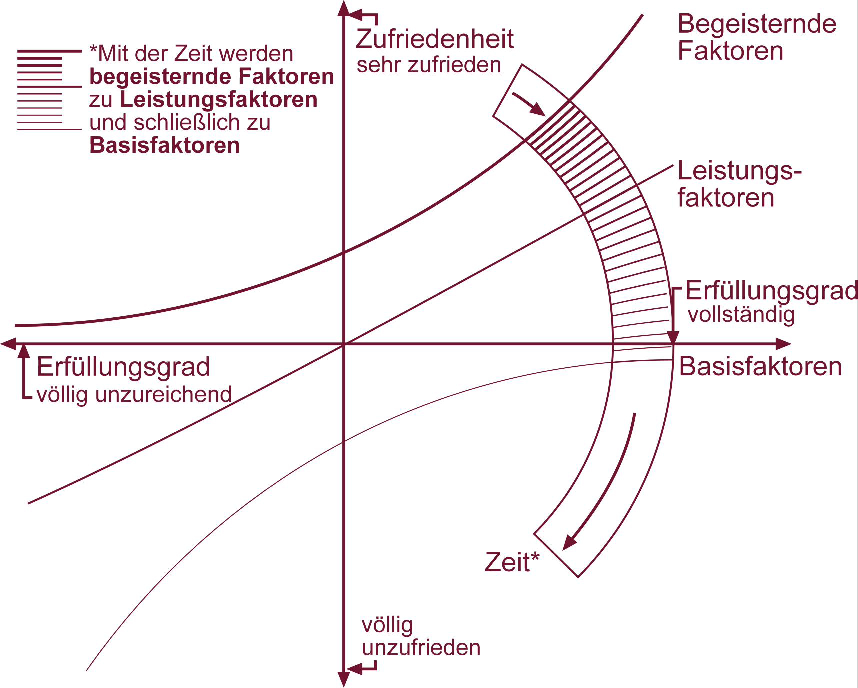
\includegraphics[width=.5\textwidth]{images/Kano-Modell.pdf}
\centering 
\captionabove[Das Kano-Modell]{Das Kano-Modell\footnotemark} 
\label{fig:kano}
\end{figure}
\footnotetext{Eine Darstellung des Kano-Modell (Quelle: \href{http://www.sophist.de/fileadmin/SOPHIST/Blog/Kano-Modell.jpg}{http://www.sophist.de/fileadmin/SOPHIST/Blog/Kano-Modell.jpg} Sichtung: 13.06.2017)} 

Doch was sind Basis-, Leistungs- und Begeisterungsfaktoren? Um ein Verständnis aufzubauen, werden diese im folgenden kurz erläutert.

\subsubsection{Basisfaktoren}
Basisfaktoren sind Features, welche von den Stakeholdern als selbstverständlich angesehen werden. Diese sollten in jedem Fall erfüllt werden, da sonst Unzufriedenheit der Kunden unvermeidbar ist. Wenn ein solches Feature fehlt, kann dies sogar dazu führen, dass ganze Stakeholder-Gruppen wegfallen.

\subsubsection{Leistungsfaktoren}
Leistungsfaktoren hingegen beschreiben Features, die bewusst von den Stakeholdern verlangt werden, jedoch nicht zwingend notwendig sind. Fehlen zu viele dieser Faktoren, hat auch das großen Einfluss auf die Zufriedenheit der Stakeholder. Wenn jedoch nur wenige dieser Faktoren fehlen, wird dies, im Gegensatz zu der Inakzeptanz bei den Leistungsfaktoren, meist geduldet und akzeptiert.

\subsubsection{Begeisterungsfaktoren}
Unter Begeisterungsfaktoren versteht man Features, welche der Kunde noch nicht kennt, deren Wert dem Nutzer allerdings während der Nutzung deutlich wird. Solche Faktoren heben das Produkt vom Markt ab und tragen erheblich zum Erfolg des Produkts bei. Meist stellen diese Faktoren ein Alleinstellungsmerkmal des Produktes dar. Doch setzt sich ein Begeisterungsfaktor auf dem Markt erst einmal durch, wird dieser nach nicht all zu langer Zeit von Stakeholdern oft als Leistungsfaktor oder sogar als Basisfaktor angesehen.\\

Ein gutes Beispiel dafür ist das Handy. Während früher mit einem Handy nur telefoniert werden konnte, hat sich irgendjemand ausgemalt wie es denn wäre, mit einem solchen Gerät auch Textnachrichten zu versenden. Dieses Feature war im ersten Moment ein Begeisterungsfaktor, denn die Nutzer kannten dieses Feature in dieser Form noch nicht. Im Laufe der Zeit haben sie es aber lieben gelernt. Kurze Zeit später wurde diese Funktion allerdings bei dem Kauf eines Handys bewusst verlangt, wodurch es dann von einem Begeisterungs- zu einem Leistungsfaktor wurde. Heute würde es sogar als Basis-Faktor eingestuft werden.

\section{Penalty-Reward-Faktoren Ansatz}
Ein anderer Ansatz Anforderungen schon bei der Ermittlung zu bewerten, ist der Penalty-Reward-Faktoren Ansatz. Hier geht es darum, die Dienstleistungsqualität einer Anforderung zu messen. Dazu werden den Anforderungen Penalty- und Reward-Faktoren zugeteilt. Penalty-Faktoren sind solche, die das Gesamturteil über ein System verschlechtern, allerdings bei einem Wegfallen auch nicht verbessern. Bei den Reward-Faktoren ist dies genau umgekehrt. Hier wird durch das Vorhandensein die Zufriedenheit der Stakeholder verbessert, das Wegfallen hat allerdings keine negative Auswirkung auf das Zielprodukt. Wie das aussehen kann, ist auf der Abbildung \ref{fig:penaltyreward} zu sehen.

\begin{figure}[!htb]
		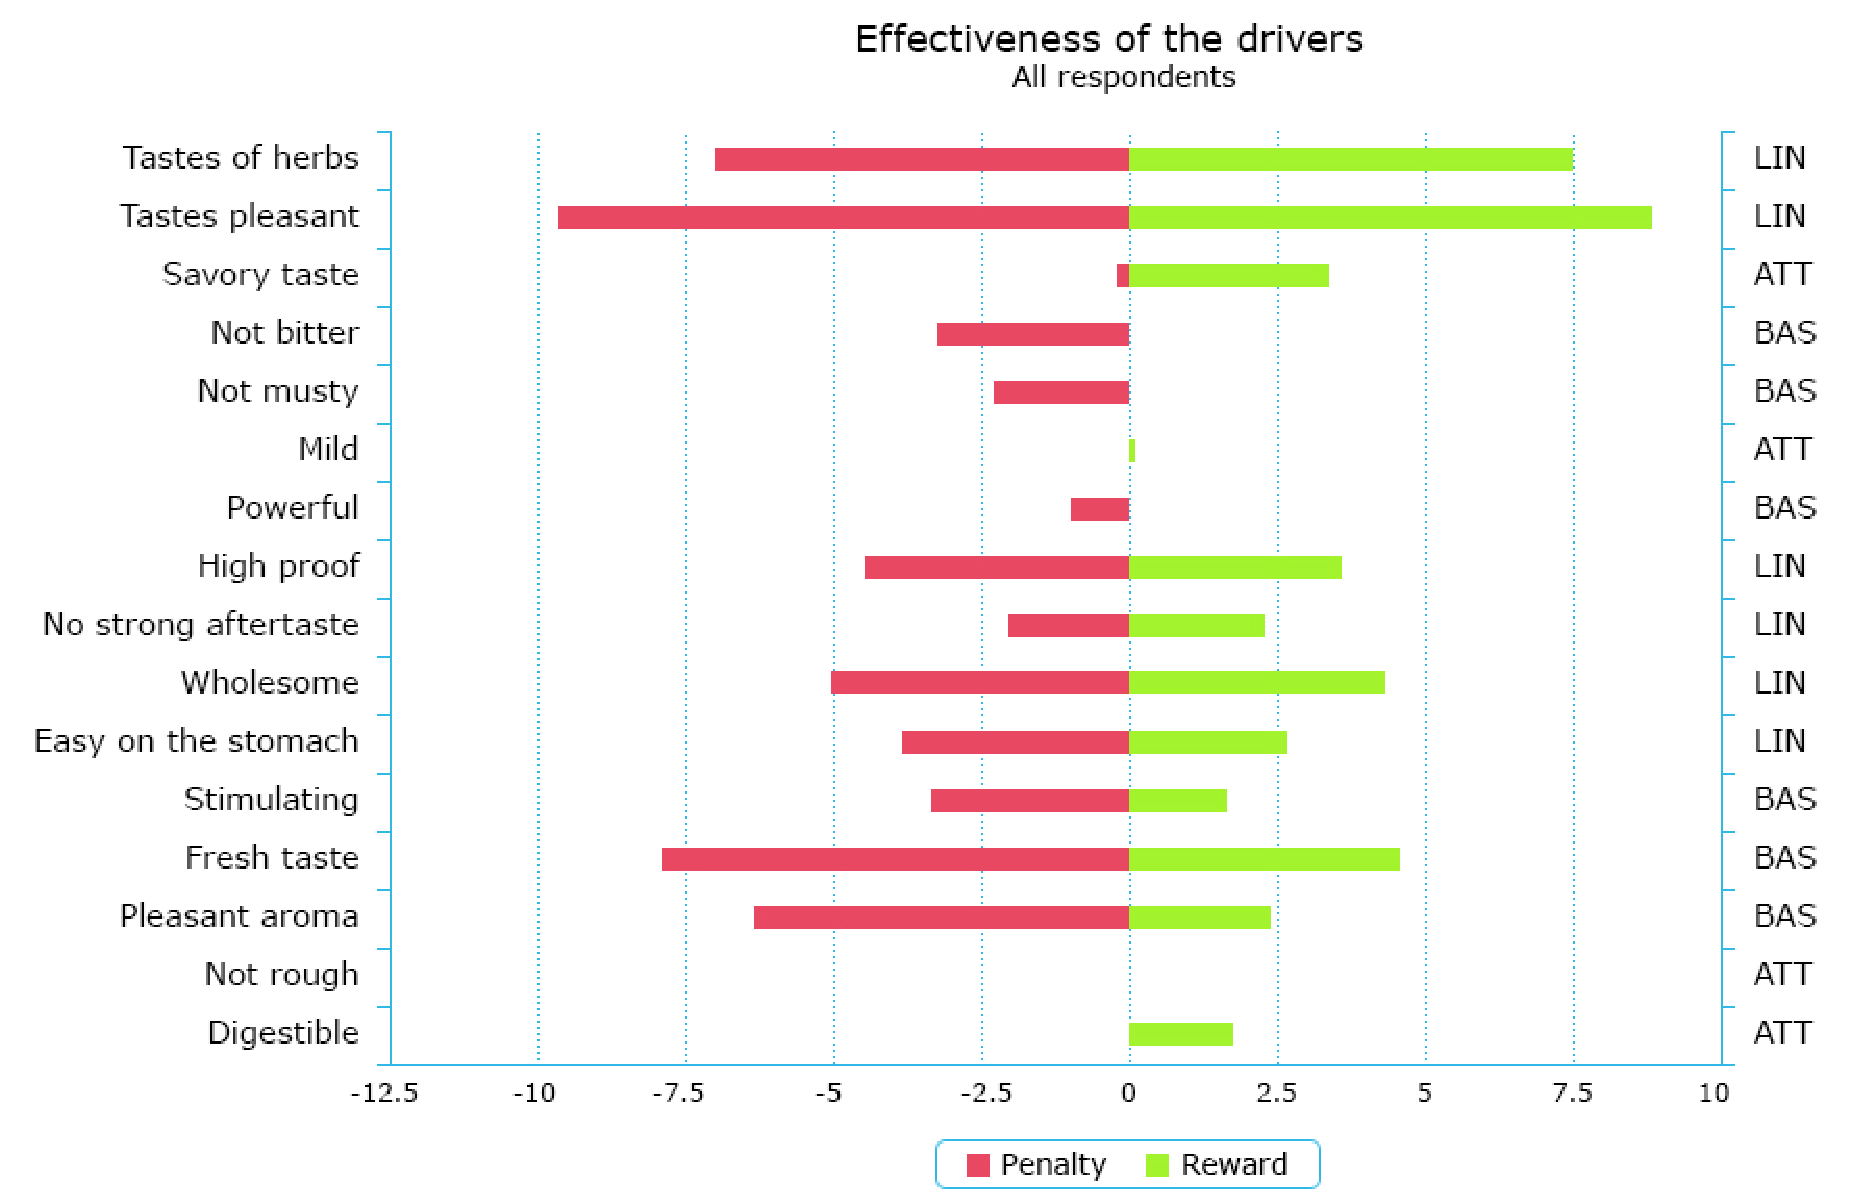
\includegraphics[width=\textwidth]{images/penaltyreward.pdf}
\centering 
\captionabove[Penalty-Reward-Analysis]{Penalty-Reward-Analysis\footnotemark} 
\label{fig:penaltyreward}
\end{figure}
\footnotetext{Eine Darstellung der Penalty-Reward-Analysis (Quelle: \href{https://www.ifad.de/services/multivariate-verfahren/neuere-ansaetze/penalty-reward-analyse-pra/?lang=en}{https://www.ifad.de/services/multivariate-verfahren/neuere-ansaetze/penalty-reward-analyse-pra/?lang=en} Sichtung: 13.06.2017)} 

\section{Anforderungen Ermitteln}
\label{subsec:ermittlung}
Wie kommt man jetzt an die Anforderungen der Stakeholder? \\
Vor der Ermittlung ist es wichtig, festzulegen, welche Art von Anforderungen man in Erfahrung bringen will. Während man bei einem \textit{"fertigen"} Produkt, möglicherweise nur neue Features und Ideen in Erfahrung bringen möchte, ist es bei einem Projekt in der Entwicklungs- oder Planungsphase durchaus wichtiger, vorerst die grundsätzlichen Wünsche und Anregungen der Stakeholder aufzunehmen. Dieser Schritt entscheidet, welche der vielen Methoden zur Ermittlung von Anforderungen eingesetzt wird. Welche Ermittlungs-Techniken es gibt, wurde von \cite{Rupp2} sehr gut und übersichtlich zusammengefasst, weshalb in dieser Arbeit nur auf den Kern dieser Methoden eingegangen wird. Grundsätzlich unterscheiden \cite{Rupp2} zwischen den Oberkategorien Kreativitäts-, Beobachtungs-, Befragungs- und artefaktbasierte Techniken. Was das ist, und wozu diese eingesetzt werden, zeigt die folgende Übersicht.

\subsection{Kreativitätstechniken}
\label{subsubsec:kreativitätstechniken}
Eine Art zur Ermittlung von Anforderungen sind Kreativitätstechniken. Diese werden eingesetzt, um neue innovative Ideen zu entwickeln. Hier versucht man aus dem herkömmlichen Denken auszubrechen, um die Tür für neue Ideen zu öffnen. Wichtig ist darauf zu achten, dass man sich vorher das richtige Umfeld schafft, um bessere Ergebnisse zu erzielen. Dann kann mit einer der folgenden Methoden der Kreativität freien Lauf gelassen werden.

\subsubsection{Brainstorming}
\label{subsubsec:brainstorming}
Die wohl bekannteste aller Kreativitätstechniken ist das Brainstorming. Dabei werden in einer Gruppe von fünf bis zehn Teilnehmern circa 20 Minuten Ideen gesammelt und vorerst ohne weitere Kommentare notiert. Anschließend werden diese Ideen sorgfältig analysiert. Durch diese Methode ist es möglich durch die Inspirationen durch Ideen anderer, eigene neue Ideen zu entwickeln.\\

Diese Technik bietet den Vorteil, dass viele Ideen in kurzer Zeit gefunden werden und die Teilnehmer diese zusammen6 entwickeln. Jedoch kann Brainstorming bei unterschiedlich dominanten Teilnehmern dazu führen, dass diese sich gegenseitig behindern. Auch ist diese Methode bei räumlich weit getrennten Stakeholdern problematisch.

\subsubsection{Brainstorming paradox}
Das Brainstorming paradox funktioniert fast genauso wie das normale Brainstorming, mit dem Unterschied, dass hier Ideen gesammelt werden, welche \textbf{nicht} erreicht werden sollen. Anschließend werden Maßnahmen entwickelt, welche diese Ideen vermeiden. \\

In manchen Situationen führt diese Methode schneller zu Ergebnissen. Auch werden so effektiv Risiken erkannt. Die Nachteile teilt sich diese Methode mit dem normalen Brainstorming.

\subsubsection{Methode 6-3-5}
Eine weitere Technik ist die Methode 6-3-5. Dabei handelt es sich um eine schriftliche Brainstorming-Methode. Hier bekommt jeder Teilnehmen einen Zettel, auf dem er innerhalb von circa fünf Minuten drei Ideen notiert. Anschließend wird dieser Zettel an den nächsten Teilnehmer weitergereicht, welcher, nachdem er die Ideen seines Kollegen durchgelesen hat, weitere drei Ideen hinzufügt. Dies wird solange wiederholt, bis jeder Teilnehmer einmal jeden Zettel hatte. Nach diesem Vorgang werden diese Ideen analysiert und zusammengefasst.\\

Da diese Technik schriftlich durchgeführt wird, lässt sie sich besonders bei einer komplizierteren Gruppendynamik einsetzen, da die in einer Diskussion aufkommenden Konflikte vermieden werden. Auch größere Distanzen zwischen den Stakeholdern können durch die Nutzung von Emails statt Zetteln bewältigt werden. Allerdings ist diese Methode, gerade durch die schriftliche Form und die zeitliche Begrenzung, nicht so effektiv wie das normale Brainstorming.

\subsubsection{Wechsel der Perspektive (6-Hut-Denken/Walt Disney-Methode)}
In manchen Situationen bietet es sich an, einen Wechsel der Perspektive vorzunehmen. Um dies zu erreichen gibt es viele verschiedene Techniken. Eine ausführliche Variante ist das \textit{6-Hut-Denken} von \textit{Edward de Bono} mit sechs Perspektiven. Diese kann man sowohl alleine als auch in Gruppen einsetzen. Die sechs Perspektiven lauten wie folgt:
\begin{enumerate}
  \setlength\itemsep{-4pt}
\item Objektivität und Neutralität
\item Persönliches Empfinden und subjektive Meinung
\item Objektive, negative Argumente
\item Objektive, positive Eigenschaften
\item Neue Ideen
\item Prozess-Kontrolle
\end{enumerate} 

Die Walt Disney-Methode ist benannt nach Walt Disney, der angeblich (so \cite{Rupp2}) für jede Sichtweise einen eigenen Raum hatte.
Hierbei wird der Stakeholder aufgefordert, jede der folgenden Perspektiven in einem anderen Raum oder zeitlich getrennt voneinander zu betrachten:

\begin{enumerate}
  \setlength\itemsep{-4pt}
\item Träumer und Visionär
\item Realist
\item Kritiker
\end{enumerate} 

Das Problem wird bei dieser Methode aus all diesen Perspektiven betrachtet, wodurch man einen sehr guten Überblick über das Gesamtbild des Projekts bekommt.\\

Mit diesen Techniken können auch Stakeholder, welche in ihrer Denkweise sehr festgefahren sind, veranlasst werden, die Dinge einmal aus einer anderen Perspektive zu betrachten. Jedoch ist es für viele schwierig sich in eine der genannten Rollen zu versetzen.

\subsubsection{Analogietechniken (Bionik/Bisoziation)}
Eine weitere Methode sind Analogietechniken. Bei einer Bionik werden als Denkmodell Analogie-Beispiele aus der Natur verwendet, um die dort gefundenen Lösungen auch auf das gegebene Problem anzuwenden. Um diesen Ansatz zu verstehen wird hier ein Beispiel von \cite{Rupp2} zitiert.

\begin{quote}
\textit{"Denken Sie zum Beispiel an die Fusion zweier Firmen und vergleichen Sie es mit dem Vermischen von zwei Tierherden. Wie lange dauert es, bis sich die Tiere der beiden Herden (die Mitarbeiter) vermischen? Die Leittiere werden in einen Konkurrenzkampf treten und eine neue Hierarchie erkämpfen. In einer Gefahrensituation, wenn zum Beispiel ein Raubtier die Herde angreift, werden sich die Tiere der beiden Tierherden als eine Herde verhalten, um ihre Chance zu verbessern, dem Raubtier zu entkommen. Diese Verhaltensmuster können in ähnlicher Form von den Mitarbeitern der beiden Firmen erwartet werden."}
\end{quote}

Bei der Bisoziation werden die Vorbilder im Gegensatz zu der Bionik nicht auf die Natur begrenzt.\\

Mit diesen Methoden ist es möglich, schwer vorstellbare Zusammenhänge oder komplexe Probleme durch den Kontextwechsel verständlich zu machen. Hierbei ist allerdings darauf zu achten, dass die verwendeten Vorbilder gut und passend ausgewählt werden. Dies nimmt unter Umständen viel Zeit in Anspruch.

\subsubsection{Osborn-Checkliste}
Die letzte der von \cite{Rupp2} aufgeführten Kreativitätstechniken ist die Osborn-Checkliste. Diese besteht aus den Punkten:
\begin{itemize}
\item Kann man das Produkt auch anders verwenden?
\item Gibt es etwas Ähnliches wie diese Produkt, und was können wir davon nachahmen?
\item Was lässt sich ändern? Kann man andere Funktionen einbauen?
\item Wie kann man das Produkt erweitern, veredeln oder teurer machen?
\item Wie kann man das Produkt vereinfachen oder auf Grundfunktionen reduzieren?
\item Kann man das Produkt oder Teile davon ersetzen?
\item Kann man das Produkt oder Teile davon umstellen, in der Reihenfolge verändern oder anders kombinieren?
\item Kann man auch das Gegenteil mit dem Produkt machen?
\item Kann man das Produkt oder die Idee mit etwas anderem kombinieren? Lässt es sich als Baustein für etwas anderes verwenden?
\item Kann man es in seiner Materie verändern? Kann man es zusammendrücken, verflüssigen, durchlöchern oder anders transformieren?
\end{itemize}

Durch die Beantwortung dieser Fragen, können gerade für ein bestehendes Produkt viele kreative Ideen gesammelt werden. Diese Methode für jede der Funktionalitäten eines großen Produkts anzuwenden kann allerdings zu aufwendig sein.

\subsection{Beobachtungstechniken}
Da aus verschiedenen Gründen nicht jeder Stakeholder in der Lage ist sein Know-how sprachlich auszudrücken, oder die Zeit hat dies zu tun, gibt es Beobachtungstechniken. Mit diesen Techniken werden Stakeholder beobachtet, um anhand ihrer Arbeitsabläufe neue Anforderungen zu entwickeln. Diese Methoden haben den Vorteil, dass sehr detaillierte Anforderungen aufgenommen werden können, da diese in der Regel von einem Fachmann selbst notiert werden.

\subsubsection{Feldbeobachtung}
Eine Beobachtungstechnik ist die Feldbeobachtung. Hierbei werden die Tätigkeiten und Arbeitsschritte der Stakeholder mit ihrem zeitlichen Zusammenhang erfasst. Unklare Arbeitsschritte können durch Fragestellungen an den Stakeholder geklärt werden.\\

Gerade für die Beobachtung unterbewusster Tätigkeiten eignet sich diese Methode sehr gut. Zudem können so leichter Abweichungen in den Prozessen analysiert werden, da der Requirements-Engineer viele Personen und ihre Tätigkeiten beobachtet. Jedoch gibt es Arbeitsabläufe die schwer bis gar nicht beobachtbar sind, diese können mit dieser Methode nicht ermittelt werden.

\subsubsection{Apprenticing}
Bei dieser Methode beobachtet der Requirements-Engineer den Stakeholder nicht, sondern erlernt die Tätigkeit, unter der Anleitung von diesem, selbst. So können die Anforderungen direkt aus der Perspektive des Stakeholders aufgenommen werden.\\

Im Gegensatz zur Feldbeobachtung fühlt sich der Stakeholder bei dieser Technik nicht beobachtet und unter Druck gesetzt. Auch bietet diese Methode psychologische Vorteile, weil der Requirements-Engineer selbst die Vor- und Nachteile eines Systems live aus der Sicht des Stakeholders erfährt.

\subsection{Befragungstechniken}
Befragungstechniken basieren darauf, Stakeholder gezielt nach ihren Wünschen und Bedürfnissen zu befragen. Für die Ermittlung von nicht-funktionalen Anforderungen ist diese Methode in den meisten Fällen nicht empfehlenswert, vielmehr wird diese dazu genutzt, funktionale Anforderungen aufzunehmen. Durch die Befragung können, je nach Umsetzung, viele neue Sichtweisen auf ein Problem erworben werden.

\subsubsection{Fragebogen}
\label{subsubsec:fragebogen}
Eine dieser Techniken ist der klassische Fragebogen. Hierfür werden eine Reihe von Fragen von den Stakeholdern, entweder online oder schriftlich, beantwortet. Diese Antworten werden anschließend ausgewertet um daraus Anforderungen zu entwickeln.\\

Mit dieser Methode kann eine große Anzahl von Stakeholdern eingebunden werden. Allerdings ist anzumerken, dass gerade implizites Wissen der Stakeholder untergeht. Auch können bei der Beantwortung dieser Fragen Unklarheiten schlecht geklärt werden, was zu einer Fehlinterpretation der Fragen führen kann.

\subsubsection{Interview}
\label{subsubsec:interview}
Bei einem Interview werden den Stakeholdern die Fragen im Gegensatz zu einem Fragebogen in einem direkten Gespräch gestellt und protokolliert. Auch hier werden diese anschließend ausgewertet und daraus Anforderungen entwickelt.\\

Der Vorteil dieser Methode ist, dass in einem offenen Gespräch oft die Hemmungen der Stakeholder gelindert werden. Des Weiteren kann der Verlauf des Gesprächs dynamisch angepasst werden. Mit dieser Technik kann besonders das Qualitätskriterium der Vollständigkeit leichter erfüllt werden als mit anderen Techniken. Jedoch sind solche Interviews sehr zeitaufwendig, was das Befragen vieler Stakeholder in den meisten Fällen erschwert.

\subsubsection{Selbstaufschreibung}
Eine weitere Form der Befragung ist die Selbstaufschreibung. Bei dieser Methode beschreibt der Stakeholder selbst Anforderungen, Änderungs- und Optimierungsvorschläge an das System. Die Qualität der Ergebnisse kann verbessert werden, indem die ausgewählten Stakeholder in die Grundlagen der Anforderungsanalyse eingewiesen werden.

Durch die Selbstaufschreibung wird der Stakeholder nicht von dem Requirements-Engineer beeinflusst. Zudem muss er sein Wissen nicht erläutern, sondern nutzt eine gleichbleibende Formulierung für seine Anforderungen.

\subsubsection{On-Site-Customer}
Anders als bei vielen anderen Methoden ist bei On-Site-Customer ein Interessenvertreter der Stakeholder während der Entwicklung ständig vor Ort. So können, besonders in einzelnen Inkrementen, die Anforderungen und deren Umsetzung optimiert werden.\\

Anforderungen werden so vor allem mündlich und sehr schnell ermittelt, dennoch ist es für viele schwierig, einen geeigneten Mitarbeiter für solche Zwecke dauerhaft zu entbehren. Auch werden bei einer fehlenden Abstimmung zwischen dem On-Site-Customer und den anderen Stakeholdern nur die Interessen einer Person vertreten.\\[1em]

\cite{Rupp2} beschreiben darüber hinaus noch Artefaktbasierte- und unterstützende Techniken zur Ermittlung von Anforderungen. Diese beziehen sich größtenteils nicht auf die Stakeholder, sondern auf existierende Systeme oder andere Quellen. Diese Art der Anforderungsermittlung entspricht nicht dem eigentlichen Sinn dieser Arbeit, weshalb diese auch nicht weiter erläutert werden.

\section{Dokumentation}
\label{subsec:dokumentation}
Um Anforderungen nach der Ermittlung bestmöglich verarbeiten zu können, ist es notwendig, diese in einem einheitlichen und fachlichen Stil zu dokumentieren. Auch hier finden sich viele Techniken dies zu tun. Einen Überblick über die wichtigsten dieser Techniken geben die folgenden Abschnitte.

\subsection{User-Storys}
Eine Möglichkeit Anforderungen zu dokumentieren sind User-Storys. Einzelne Systemfunktionalitäten werden in kleine Storys verpackt, welche aus der Sicht des Users formuliert sind. Diese dienen in wenigen Sätzen als Gedankenstütze zu der Anforderung. Eine User-Story könnte wie folgt lauten:

\begin{quote}
\textit{"Als Mitarbeiter möchte ich Urlaub vorab über ein elektronisches Formular beantragen können, damit ich eine offizielle Genehmigung erhalte um dann eine Ferienreise verbindlich buchen zu können."}
\end{quote}

User-Storys bilden zwar neben der eigentlichen Anforderung auch die Intention des Users ab, jedoch sind diese teilweise für die Entwickler schwieriger zu implementieren, da sie meist dafür zu grob formuliert sind.

\subsection{Use-Cases}
Ähnlich wie bei User-Storys bilden Use-Cases die Anforderung aus der Sicht des Users ab, diese sind aber in den meisten Fällen wesentlich grober formuliert. Auch werden hier oft sogar nur einzelne Aktionen beschrieben. Einige Beispiele dazu könnten lauten:
\begin{quote}
\textit{"Geld abheben"}
\textit{"Überweisung tätigen"} oder
\textit{"Kontostand überprüfen"}
\end{quote}

\subsection{Technical Storys}
Da Anforderungen nicht immer nur Funktionalitäten beschreiben, sondern manchmal auch technische Details, können diese gegebenenfalls nicht in User-Storys beschreiben werden. Um diese dennoch zu betrachten, werden Technical Storys verwendet. Diese sind im Prinzip nichts anderes als User-Storys, welche aus technischer Sicht eine nicht-funktionale Anforderung beschreiben.

\subsection{FunctionsMASTeR}
\label{subsec:functionmaster}
Eine weitere Alternative zur Dokumentation von Anforderungen beschrieben \cite{SOPHIST2}. Hierbei dient eine ganz einfach Schablone dazu, die wichtigsten Informationen einer Anforderung in einen Satz zu verpacken. Diese Schablone sieht wie folgt aus:

\textit{<System> <muss,sollte,wird>} \textit{<Akteur>, fähig sein} \textit{<Objekt> <Prozesswort>}\\

Diese Methode hat den Vorteil, dass so nicht nur funktionale, sondern auch nicht-funktionale Anforderungen, dokumentiert werden können. Auch ist diese Form der Beschreibung für die Entwickler gut interpretierbar.

\section{Validation}
Die Validation ist ein wichtiger Schritt im \acl{RE}. Nachdem die Anforderungen dokumentiert wurden muss geprüft werden, ob diese auch tatsächlich umsetzbar sind. Es kann vorkommen, dass Anforderungen über den Funktionsrahmen des Systems hinaus gehen und somit vorerst nicht mehr in Betracht gezogen werden. Dieser Schritt stellt also eine Überprüfung aller Anforderungen dar, wobei nicht valide Anforderungen aussortiert werden. Dies kann in Zusammenarbeit mit dem Entwickler-Team oder dem Product-Owner geschehen.  

\section{Auswertung}
Die ermittelten Anforderungen müssen vor der eigentlichen Implementierungsarbeit ausgewertet werden. Das sorgt für eine detailliertere Priorisierung. So kann ein Plan erstellt werden, ob und in welcher Reihenfolge diese erfüllt werden. Die bekanntesten Methoden eine Auswertung durchzuführen werden im folgenden Abschnitt kurz erklärt.

\subsection{Function-Point-Analyse}
Mit der \ac{FPA} wird der Aufwand einzelner Anforderungen oder Anforderungsgruppen gemessen. Dieser Aufwand wird in Function-Points angegeben. Bei dieser Methode werden (so \cite{Lipinski}) in drei Stufen die sogenannten unbewerteten oder auch unjustierten \ac{FP} bestimmt. Dazu werden in der ersten Stufe Parameter wie: Anzahl der Benutzer- Eingaben und Ausgaben, Anzahl der Benutzerabfragen, Anzahl der Datenbankspalten und die Anzahl der Schnittstellen zu externen Systemen in die Berechnung mit einbezogen. Die so errechneten \ac{FP} werden anschließend in der zweiten und dritten Stufe durch Komplexitätsparameter und Konstanten des Entwicklungsprozesses gewichtet. Anschließend werden den Anforderungen Werte für bestimmte Charakteristika, wie die Wiederverwertbarkeit, zugewiesen. \\

Nach diesen drei Stufen spricht man von bewerteten oder auch justierten \ac{FP}. Diese werden, um eine Aussage über den Implementierungsaufwand treffen zu können, anschließend mit Erfahrungswerten und der Produktivität von Software-Entwicklungsprozessen verglichen und in Mitarbeiter-Monate umgerechnet. Mitarbeiter-Monate geben an, wie viele Monate ein Mitarbeiter für die Umsetzung benötigt.\\

Diese Methode beruht zwar im Gegensatz zu anderen Methoden größtenteils nicht auf Schätzungen sondern auf Fakten und Erfahrungswerten, jedoch ist die Ermittlung des Aufwands mit dieser Technik sehr zeitaufwendig und komplex. Auch zeigt laut der \cite{AGIL1} die Erfahrung, dass das vergleichende Schätzen, wie es bei Story-Points durchgeführt wird, zu deutlich schnelleren und besseren Ergebnissen führt.

\subsection{Story-Points}
Eine Aufwandsschätzung mit Story-Points ist wesentlich schneller als der langwierige Prozess der Function-Point-Analyse und stellt deshalb vor allem in agilen Projekten eine gern gesehene Alternative dar. Hierzu werden den zuvor erstellten User-Storys Story-Points zugewiesen, welche eine abstrakte Komplexität der einzelnen Storys angibt. Dabei wird eine Skala festgelegt, in welcher die Story-Points vergeben werden. \cite{Preuss1} empfiehlt als Skala eine abgeänderte Form der Fibonacci-Folge zu verwenden, welche aus den Elementen 1, 2, 3, 5, 8, 13, 20, 40 und 100 besteht. User-Storys mit vielen Story-Points bedeuten, dass diese Story in kleinere Storys aufgeteilt werden muss, um realistisch abgeschätzt werden zu können. Man kann allerdings auch eine einfache Skala von beispielsweise 1-10 nutzen.\\

Nach der Festlegung dieser Skala wird eine Story ausgesucht, die einen guten Mittelwert an Komplexität mit sich bringt. An dieser Story wird sich bei der Vergabe weiterer Story-Points orientiert. \\[1em]

Es gibt noch weitere Methoden zur Aufwandsschätzung einer Anforderung, wie beispielsweise das CoCoMo (mehr dazu auf \cite{COCOMO}), die COSMIC-Methode der \cite{COSMIC}, Lines of Code, Ad-hoc-Schätzmethoden oder umfangbasierte Schätzmethoden. Eine gute Übersicht über diese Methoden bietet das \cite{WinfWiki}.


%======================================================================
%======================================================================
% Eintrag ins Glossar
\nomenclature{Requirement-Engineering}{Der Prozess der Ermittlung, Analyse, Auswertung und Bearbeitung von Anforderungen.\vspace{4mm}}

\nomenclature{Requirement-Engineer}{Die Person, welche das Requirement-Engineering durchführt.\vspace{4mm}}

\nomenclature{System}{System wird im Kontext dieser Arbeit als Synonym für das zu entwickelnde System eingesetzt.\vspace{4mm}}

\nomenclature{Produkt}{Ein weiteres Synonym für das zu entwickelnde System.\vspace{4mm}}

\nomenclature{Projekt}{Der Prozess zur Planung und Entwicklung eines Systems.\vspace{4mm}}

\nomenclature{Usability}{Das Ausmaß, in dem ein Produkt durch bestimmte Benutzer in einem Nutzungskontext benutzt werden kann, um ein Ziel effektiv, effizient und zufriedenstellend zu erreichen.\vspace{4mm}}

\nomenclature{Funktion-Points}{Ein Maß für den Aufwand der Umsetzung einer Funktionalität. Diese finden Anwendung in der Function-Point-Analyse\vspace{4mm}}

\nomenclature{User-Story}{Eine Art Anforderungen aus der Sicht des Nutzer zu dokumentieren.\vspace{4mm}}

\nomenclature{Story-Points}{Ein Maß zur Angabe der Komplexität einer User-Story.\vspace{4mm}}

\nomenclature{Use-Cases}{Eine Art Funktionalitäten die ein System bieten soll zu beschreiben.\vspace{4mm}}

\nomenclature{User}{Der Nutzer eines Systems.\vspace{4mm}}

\nomenclature{Potentieller Nutzer}{Ein möglicher zukünftiger Nutzer eines Systems.\vspace{4mm}}